%%%%%%%%%%%%%%%%%%%%%%%%%%%%%%%%%%%%%%%%%
% Beamer Presentation
% LaTeX Template
% Version 1.0 (10/11/12)
%
% This template has been downloaded from:
% http://www.LaTeXTemplates.com
%
% License:
% CC BY-NC-SA 3.0 (http://creativecommons.org/licenses/by-nc-sa/3.0/)
%
%%%%%%%%%%%%%%%%%%%%%%%%%%%%%%%%%%%%%%%%%

%----------------------------------------------------------------------------------------
%	PACKAGES AND THEMES
%----------------------------------------------------------------------------------------

\documentclass{beamer}

\mode<presentation> {

% The Beamer class comes with a number of default slide themes
% which change the colors and layouts of slides. Below this is a list
% of all the themes, uncomment each in turn to see what they look like.

%\usetheme{default}
%\usetheme{AnnArbor}
%\usetheme{Antibes}
%\usetheme{Bergen}
%\usetheme{Berkeley}
%\usetheme{Berlin}
%\usetheme{Boadilla}
%\usetheme{CambridgeUS}
%\usetheme{Copenhagen}
%\usetheme{Darmstadt}
%\usetheme{Dresden}
%\usetheme{Frankfurt}
%\usetheme{Goettingen}
%\usetheme{Hannover}
%\usetheme{Ilmenau}
%\usetheme{JuanLesPins}
%\usetheme{Luebeck}
\usetheme{Madrid}
%\usetheme{Malmoe}
%\usetheme{Marburg}
%\usetheme{Montpellier}
%\usetheme{PaloAlto}
%\usetheme{Pittsburgh}
%\usetheme{Rochester}
%\usetheme{Singapore}
%\usetheme{Szeged}
%\usetheme{Warsaw}

% As well as themes, the Beamer class has a number of color themes
% for any slide theme. Uncomment each of these in turn to see how it
% changes the colors of your current slide theme.

%\usecolortheme{albatross}
%\usecolortheme{beaver}
%\usecolortheme{beetle}
%\usecolortheme{crane}
%\usecolortheme{dolphin}
%\usecolortheme{dove}
%\usecolortheme{fly}
%\usecolortheme{lily}
%\usecolortheme{orchid}
%\usecolortheme{rose}
%\usecolortheme{seagull}
%\usecolortheme{seahorse}
%\usecolortheme{whale}
%\usecolortheme{wolverine}

%\setbeamertemplate{footline} % To remove the footer line in all slides uncomment this line
%\setbeamertemplate{footline}[page number] % To replace the footer line in all slides with a simple slide count uncomment this line

%\setbeamertemplate{navigation symbols}{} % To remove the navigation symbols from the bottom of all slides uncomment this line
}

\usepackage{graphicx} % Allows including images
\usepackage{booktabs} % Allows the use of \toprule, \midrule and \bottomrule in tables
\usepackage{cool}

%----------------------------------------------------------------------------------------
%	TITLE PAGE
%----------------------------------------------------------------------------------------

\title[Efficient Frontier Mathematics]{A Quick/Terse Intro to Efficient Frontier Mathematics} % The short title appears at the bottom of every slide, the full title is only on the title page

\author{Ashwin Rao} % Your name
% \institute[Ashwin Rao] % Your institution as it will appear on the bottom of every slide, may be shorthand to save space
{
% Your institution for the title page
}

\date{\today} % Date, can be changed to a custom date

\begin{document}
\begin{frame}
\titlepage % Print the title page as the first slide
\end{frame}

\begin{frame}
\frametitle{Overview} % Table of contents slide, comment this block out to remove it
\tableofcontents % Throughout your presentation, if you choose to use \section{} and \subsection{} commands, these will automatically be printed on this slide as an overview of your presentation
\end{frame}

\section{Setting and Notation}

\begin{frame}
\frametitle{Setting and Notation}
\begin{itemize}
\item $n$ assets in the economy with usual regularity/idealistic conditions
\item Their mean returns denoted by column $n$-vector $R$
\item Their covariance of returns denoted by $V$ ($n \times n$ non-singular matrix)
\item Column $n$-vector $X_p$ denotes proportions of $n$ assets in portfolio $p$
\item Denote $1_n$ as a column $n$-vector of all 1's
\end{itemize}
$$X_p^T \cdot 1_n = 1$$
We drop subscript $p$ whenever the reference to portfolio $p$ is clear
\end{frame}

\begin{frame}
\frametitle{Portfolio Returns}
\begin{itemize}
\item A single portfolio's mean return is $X^T \cdot R$
\item A single portfolio's variance of return is the quadratic form $X^T \cdot V \cdot X$
\item Covariance between portfolios $p$ and $q$ is the bilinear form $X_p^T \cdot V \cdot X_q$
\item Covariance of assets with a single portfolio is $V \cdot X$ ($n$-vector)
\end{itemize}
\end{frame}

\section{Derivation of Efficient Frontier Curve}

\begin{frame}
\frametitle{Derivation of Efficient Frontier Curve}
\begin{itemize}
\item Efficient frontier is defined for a world with no risk-free assets
\item It is the set of portfolios with minimum variance of return for each level of portfolio mean returns
\item So, minimize portfolio variance $X^T \cdot V_p \cdot X$ subject to constraints:
\end{itemize}
$$X^T \cdot 1_n = 1$$
$$X^T \cdot R = r_p$$
where $r_p$ is the mean return for efficient portfolio $p$.
\begin{itemize}
\item Set up the Lagrangian and solve to express $X$ in terms of $R, V, r_p$ 
\item Substituting for $X$ gives us the efficient frontier parabola:
\end{itemize}
$$\sigma_p^2 = \frac {a - 2 b r_p + c r_p^2} {ac - b^2} \mbox{ where}$$
$$a = R^T \cdot V^{-1} \cdot R, b = R^T \cdot V^{-1} \cdot 1_n, c = 1_n^T V^{-1} 1_n$$
\end{frame}

\begin{frame}
\frametitle{The Efficient Frontier with 16 assets}
\begin{figure}
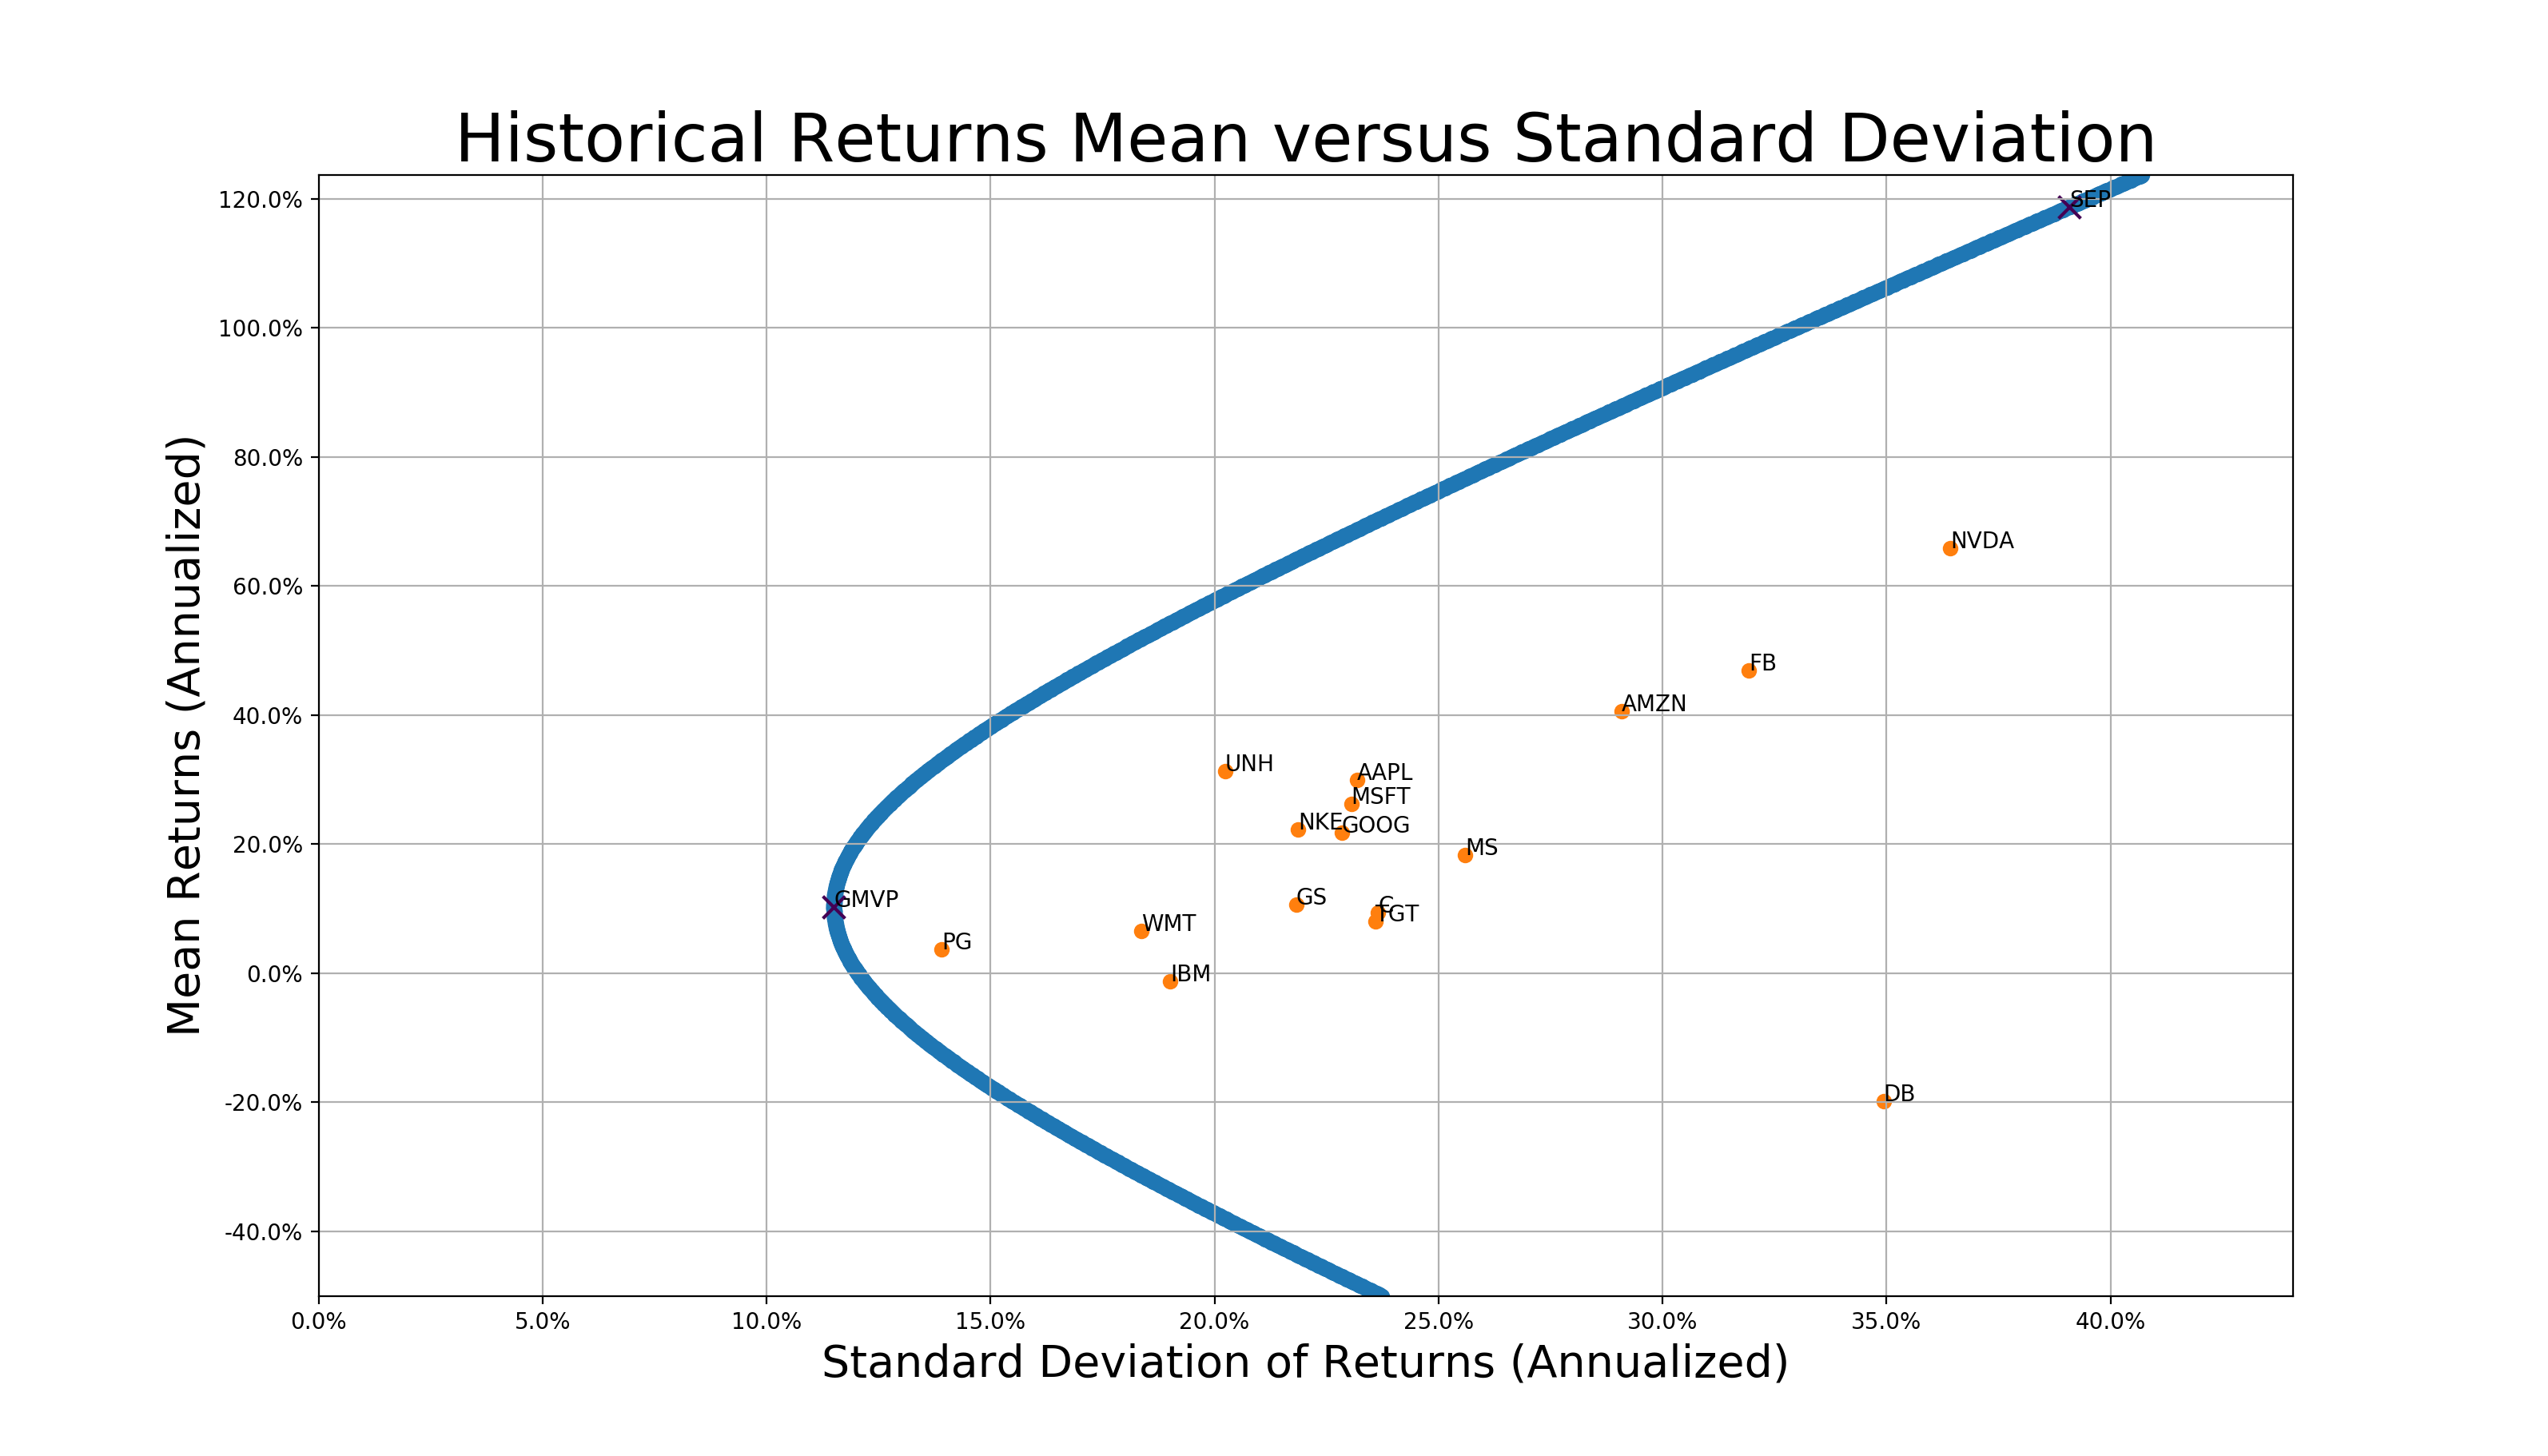
\includegraphics[scale=0.32]{EffFront.png}
\end{figure}
\end{frame}

\section{Interesting Efficient Portfolios}
\begin{frame}
\frametitle{Global Minimum Variance Portfolio (GMVP)}
\begin{itemize}
\item Global minimum variance portfolio (GMVP) is the tip of the curve
\item It has mean $r_0 = \frac b c$
\item It has variance $\sigma_0^2 = \frac 1 c$
\item It has investment proportions $X_0 = \frac {V^{-1} \cdot 1_n} c$
\item GMVP is positively correlated with all portfolios and assets
\item GMVP's covariance with all assets and all portfolios is a constant $\sigma_0^2$ (which is also equal to its own variance)
\end{itemize}
\end{frame}

\begin{frame}
\frametitle{Orthogonal Efficient Portfolios}
For every efficient portfolio $p$ (other than GMVP), there exists a unique orthogonal efficient portfolio $z$ (i.e. $Covariance(p,z) = 0$) with finite mean
$$r_z = \frac {a - b r_p} {b - c r_p}$$
\begin{itemize}
\item $z$ always lies on the opposite side of $p$ on the efficient frontier
\item  In mean-variance space, the straight line from $p$ to GMVP intersects the mean axis at  $r_z$
\item In mean-stdev space, the tangent to the efficient frontier at $p$ intersects the mean axis at $r_z$
\item All portfolios on one side of the efficient frontier are positively correlated with each other
\end{itemize}
\end{frame}

\begin{frame}
\frametitle{Two-fund Theorem}
\begin{itemize}
\item The $X$ vector of any efficient portfolio is a linear combination of the $X$ vectors of two other efficient portfolios
\item Notationally, $X_p = \alpha X_{p_1} + (1-\alpha) X_{p_2}$ for some scalar $\alpha$
\item The range of $\alpha$ from $-\infty$ to $+\infty$ traces the efficient frontier
\item So to construct all efficient portfolios, we just need to identify two canonical efficient portfolios
\item One of them is GMVP
\item The other is a portfolio we call Special Efficient Portfolio (SEP) with:
\begin{itemize}
\item Mean $r_1  = \frac a b$
\item Variance $\sigma_1^2 = \frac a {b^2}$
\item Investment proportions $X_1 = \frac {V^{-1} \cdot R} {b}$
\end{itemize}
\item The orthogonal portfolio to SEP has mean $r_z = \frac {a - b \frac a b} {b - c \frac a b} = 0$
\end{itemize}
\end{frame}


\section{Linearity of Covariance Vector w.r.t. Mean Returns (a.k.a. CAPM)}

\begin{frame}
\frametitle{Linearity of Covariance Vector w.r.t. Mean Returns}

{\bf Important Theorem}: The covariance vector of individual assets with a portfolio ( = V X) can be expressed as an exact linear function of the individual mean returns vector iff the portfolio is efficient. If the efficient portfolio is $p$ (and its orthogonal portfolio $z$), then:

$$R = r_z 1_n + \frac {r_p - r_z} {\sigma_p^2} CovarianceVector_p$$
$$ = r_z 1_n + \frac {r_p - r_z} {\sigma_p^2} (V \cdot X_p) = r_z 1_n +  (r_p - r_z) \beta_p$$

where $\beta_p = \frac {CovarianceVector_p} {\sigma_p^2}$ is the vector of slope coefficients of regressions where the explanatory variable is the portfolio return and the $n$ dependent variables are the asset returns.

The linearity of $\beta$s w.r.t. mean returns is the (in)famous CAPM banner.
\end{frame}

\begin{frame}
\frametitle{Useful Corollaries}
\begin{itemize}
\item If $p$ is SEP, $r_z = 0$ which would mean: $R = r_p \beta_p = \frac {r_p} {\sigma_p^2} V \cdot X_p$
\item So, in this case, covariance vector and $\beta_p$ are just scalar multiples of asset mean vector
\item The investment proportion $X$ in a given individual asset changes monotonically along the efficient frontier
\item $Covariance = V \cdot X$ is also monotonic along the efficient frontier
\item But $\beta$ is not monotonic $\Rightarrow$ For every individual asset, there is a unique pair of efficient portfolios that result in max and min $\beta$s for that asset
\end{itemize}
\end{frame}

\begin{frame}
\frametitle{Cross-Sectional Variance}
\begin{itemize}
\item The cross-sectional variance in $\beta$s (variance in $\beta$s across assets for a fixed efficient portfolio) is zero when efficient portfolio is GMVP and when efficient portfolio has infinite mean
\item The cross-sectional variance in $\beta$s is maximum for the two efficient portfolios with means: $ r_0 \pm \sigma_0^2 \sqrt{|A|}$ where $A$ is the 2 $\times$ 2 matrix consisting of $a,b,b,c$
\item These two portfolios lie symmetrically on opposite sides of the efficient frontier (their $\beta$s are equal and of opposite signs), and are the only two orthogonal efficient portfolios with the same variance ( $= 2 \sigma_0^2$)
\end{itemize}
\end{frame}

\section{Efficient Set with a Risk-Free Asset}

\begin{frame}
\frametitle{Efficient Set with a Risk-Free Asset}
\begin{itemize}
\item If we have a risk-free asset with return $r_F$, $V$ is singular
\item  First form the efficient frontier without the risk-free asset
\item The efficient set (with a risk-free asset) is the tangent to the efficient frontier (without the risk-free asset) in mean-stdev space from $(0, r_F)$
\item Let tangency point portfolio be $T$ with return $r_T$
\item If $r_F < r_0, r_T > r_F$
\item If $r_F > r_0, r_T < r_F$
\item All portfolios on this efficient set are perfectly correlated
\item Homework: How is $T$ related to SEP?
\end{itemize}
\end{frame}

\end{document}